\documentclass[journal]{IEEEtran}
\usepackage[a5paper, margin=10mm, onecolumn]{geometry}
%\usepackage{lmodern} % Ensure lmodern is loaded for pdflatex


\setlength{\headheight}{1cm} % Set the height of the header box
\setlength{\headsep}{0mm}     % Set the distance between the header box and the top of the text

\usepackage{gvv-book}
\usepackage{gvv}
\usepackage{cite}
\usepackage{amsmath,amssymb,amsfonts,amsthm}
\usepackage{algorithmic}
\usepackage{graphicx}
\usepackage{textcomp}
\usepackage{xcolor}
\usepackage{txfonts}
\usepackage{listings}
\usepackage{enumitem}
\usepackage{mathtools}
\usepackage{gensymb}
\usepackage{comment}
\usepackage[breaklinks=true]{hyperref}
\usepackage{tkz-euclide} 
\usepackage{listings}
% \usepackage{gvv}                                        
\def\inputGnumericTable{}                                 
\usepackage[latin1]{inputenc}                                
\usepackage{color}                                            
\usepackage{array}                                            
\usepackage{longtable}                                       
\usepackage{calc}                                             
\usepackage{multirow}                                         
\usepackage{hhline}                                           
\usepackage{ifthen}                                           
\usepackage{lscape}
\begin{document}

\bibliographystyle{IEEEtran}
\vspace{3cm}

\title{10.4.3.1.2}
\author{EE24BTECH11033 - Kolluru Suraj}
 \maketitle
% \newpage
% \bigskip
{\let\newpage\relax\maketitle}

\renewcommand{\thefigure}{\theenumi}
\renewcommand{\thetable}{\theenumi}
\setlength{\intextsep}{10pt} % Space between text and floats


\numberwithin{equation}{enumi}
\numberwithin{figure}{enumi}
\renewcommand{\thetable}{\theenumi}


\textbf{Question}:\\
Find the roots of the equation $2x^2+x-4=0$
\\
\textbf{Solution: }\\
Theoritical solution:\\

Applying quadratic formula gives solution as
\begin{align}
	x_1 = \frac{-1-\sqrt{33}}{4}\\
	x_2 = \frac{-1+\sqrt{33}}{4}
\end{align}
Computational solution:\\
We can solve the above equation using fixed point iterations. First we separate $x$, from the above equation and make an update equation of the below sort.
\begin{align}
	x = g\brak{x} = \frac{4-2x^2}{2}
\end{align}
Applying the above update equation on our equation, we get
\begin{align}
	x_{n+1}=\frac{4-2x^2_n}{2}
\end{align}
Now we start with an initial guess $x_0 = 10 $\\
But we realize that the updated values always approach infinity for any initial value. \\
So we will use Newton-Rapshon method\\
\textbf{Newton-Raphson Method:}\\
Start with an initial guess $x_0$, and then run the following logical loop,
\begin{align}
    x_{n+1} = x_n - \frac{f\brak{x_n}}{f^{\prime}\brak{x_n}} 
\end{align}
where,
\begin{align}
    f\brak{x} = 2x^2 + x + -4\\
    f^{\prime}\brak{x} = 4x+1
\end{align}
The update equation will be
\begin{align}
	x_{n+1} = x_n - \frac{2{x_n}^2 + x_n - 4}{4x_n+1}\\
\end{align}
The problem with this method is if the roots are complex but the coeffcients are real, $x_n$ either converges to an extrema or grows continuously without any bound.
To get the complex solutions, however , we can just take the initial guess point to be a 
random complex number.\\
The output of a program written to find roots is shown below:
\begin{align}
	r_1 =-1.6861 \\
	r_2 = 1.1859
\end{align}
\textbf{CODING LOGIC FOR FINDING EIGENVALUES :-}\\


The quadratic equation 
\begin{align}
2x^2+x-4=0
\end{align}
is rewritten in matrix form:
\begin{align}
\text{Matrix} =
\myvec{0 & -\frac{c}{a} \\
1 & -\frac{b}{a}
}
\end{align}

\begin{align}
a = 2, \quad b=1, \quad c = -4.
\end{align}

Substituting the values of $a,b$ and $c$, the matrix becomes:\\
Let
\begin{align}
\text{A} =
\myvec{0 & 2 \\
1 & -\frac{1}{2}
}
\end{align}




\textbf{QR-Algorithm}\\
The QR method is an iterative algorithm used to compute the eigenvalues of a square matrix $A$. The algorithm works as follows:
\begin{enumerate}
    
\item Initialization \\
Let $A_0 = A $, where $A$ is the given matrix.

\item QR Decomposition \\
For each iteration $ k = 0, 1, 2, \dots $:
\begin{enumerate}
    \item Compute the QR decomposition of \( A_k \), such that:
    \begin{align}
    A_k = Q_k R_k
    \end{align}
    where:
    \begin{enumerate}
        \item $Q_k $ is an orthogonal matrix ($ Q_k^\top Q_k = I $).
        \item $ R_k $ is an upper triangular matrix.
    \end{enumerate}
    The decomposition ensures $ A_k = Q_k R_k $.

    \item Form the next matrix \( A_{k+1} \) as:
    \begin{align}
    A_{k+1} = R_k Q_k
    \end{align}
\end{enumerate}

\item Convergence\\
Repeat Step 2 until $ A_k $ converges to an upper triangular matrix $ T $. The diagonal entries of $T$ are the eigenvalues of $A$.\\
\item The eigenvalues of matrix will be the roots of the equation.\\
The roots we get by using this method are 
\begin{align}
    x_1=1.18614066\\
    x_2=-1.68614066
\end{align}
\end{enumerate}
\begin{figure}[!ht]
    \centering
    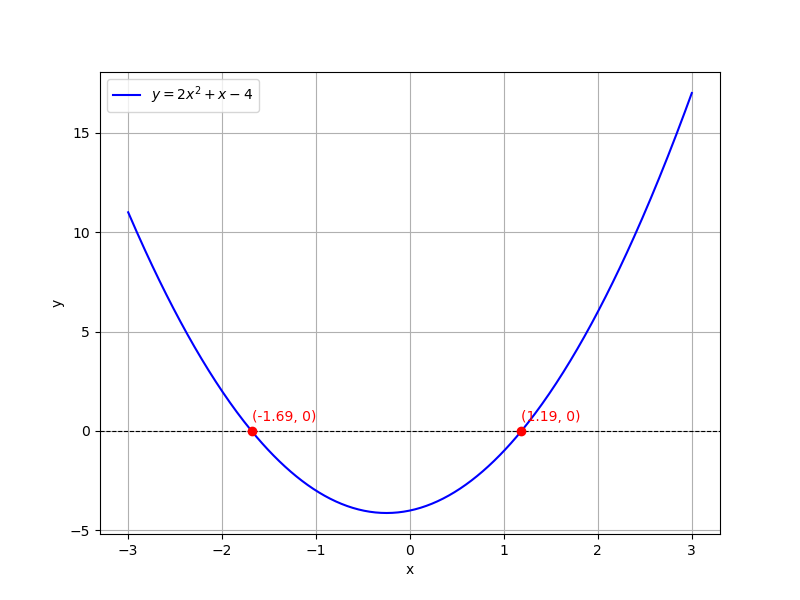
\includegraphics[width=\columnwidth]{figs/Figure_1.png}
    \caption{}
\end{figure}
\end{document}

